\glsresetall
\chapter{State of the Art}
\label{chap:state_of_the_art}

In this Chapter, we discuss the core concepts regarding the project, the most modern technology for the purpose today and related work in the area. All the information presented results from work of research through published articles, knowledge exchange and web searching.

First, the main purpose of Section~\ref{sec:concepts}~-~\nameref{sec:concepts} is to introduce and provide a brief explanation about the core concepts to the reader. Second, Section~\ref{sec:technologies}~-~\nameref{sec:technologies}, all the relevant technologies are analysed and discussed. In the final Section~\ref{sec:related_work}~-~\nameref{sec:related_work}, published articles and posts of related work are presented and possible research directions are discussed.

\section{Concepts}
\label{sec:concepts}

The following concepts represents the baseline to understand the work related to this research project. First an explanation of higher level of concepts that composes the title of this thesis are presented in Subsections~\ref{subsec:microservices} and~\ref{subsec:observability_and_controlling_performance}. The following Subsections~\ref{subsec:distributed_tracing} to~\ref{subsec:time_series}, aim to cover topics  related to previous concepts:~\nameref{subsec:distributed_tracing}, ~\nameref{subsec:graphs} and~~\nameref{subsec:time_series}.

\subsection{Microservices}
\label{subsec:microservices}

The term ``micro web services'' was first used by Dr. Peter Rogers during a conference on cloud computing in 2005, and evolved later on to ``Microservices'' at an event for software architects in 2011, where the term was used to describe a style of architecture that many attendees were experimenting with at the time. Netflix and Amazon were among the early pioneers of microservices~\cite{MauersbergerMicroservices}.

Microservices is ``an architectural style that structures an application as a collection of loosely coupled services, which implement business capabilities''~\cite{Dragoni2017, microservices_definition}.

This style of software development has a very long history and has being introduced and evolving due to software engineering achievements in the later years regarding cloud distributed computing infrastructures, \gls{api} improvements, agile development methodologies and the emergence of the recent phenomenon of containerized applications. ``A container is a standard unit of software that packages up code and all its dependencies so the application runs quickly and reliably from one computing environment to another, communicating with others through an \gls{api}''~\cite{Pahl2017}.

In Microservices, services are small, specifically calibrated to perform a single function, also each service is designed to be autonomous, resilient, minimal and composable. This framework brings a culture of rapid iteration, automation, testing, and continuous deployment, enabling teams to create products and deploy code exponentially faster than ever before~\cite{Newman}.

%The core concept of microservices stands in isolation, or by other words, what everyone wants to achieve when building a software with microservices in mind, is to share less things between the services and deal with correlated failures. In this sense, a service is a small part of the entire system (e.g. Get messages microservice), and represents a tiny feature of the whole service (e.g. Chat Service). To do this, normally every microservice is encapsulated inside a container (e.g. Docker container~\cite{docker}), and each runs in its own process and communicates with the other using lightweight mechanisms, often an \gls{http} resource \gls{api}. 

Until the rising of Microservices based architecture, the Monolithic architectural style was the most used. This style has a the particularity of produce software composed all in one piece. All features are bundled, packaged and deployed in a single tier application using a single code base.

Figure~\ref{fig:monolithic_and_microservices} aims to give a comparison between both architectural styles, Monolithic and Microservices, and provide an insight about the differences between them.

\begin{figure}[H]
    \centering
    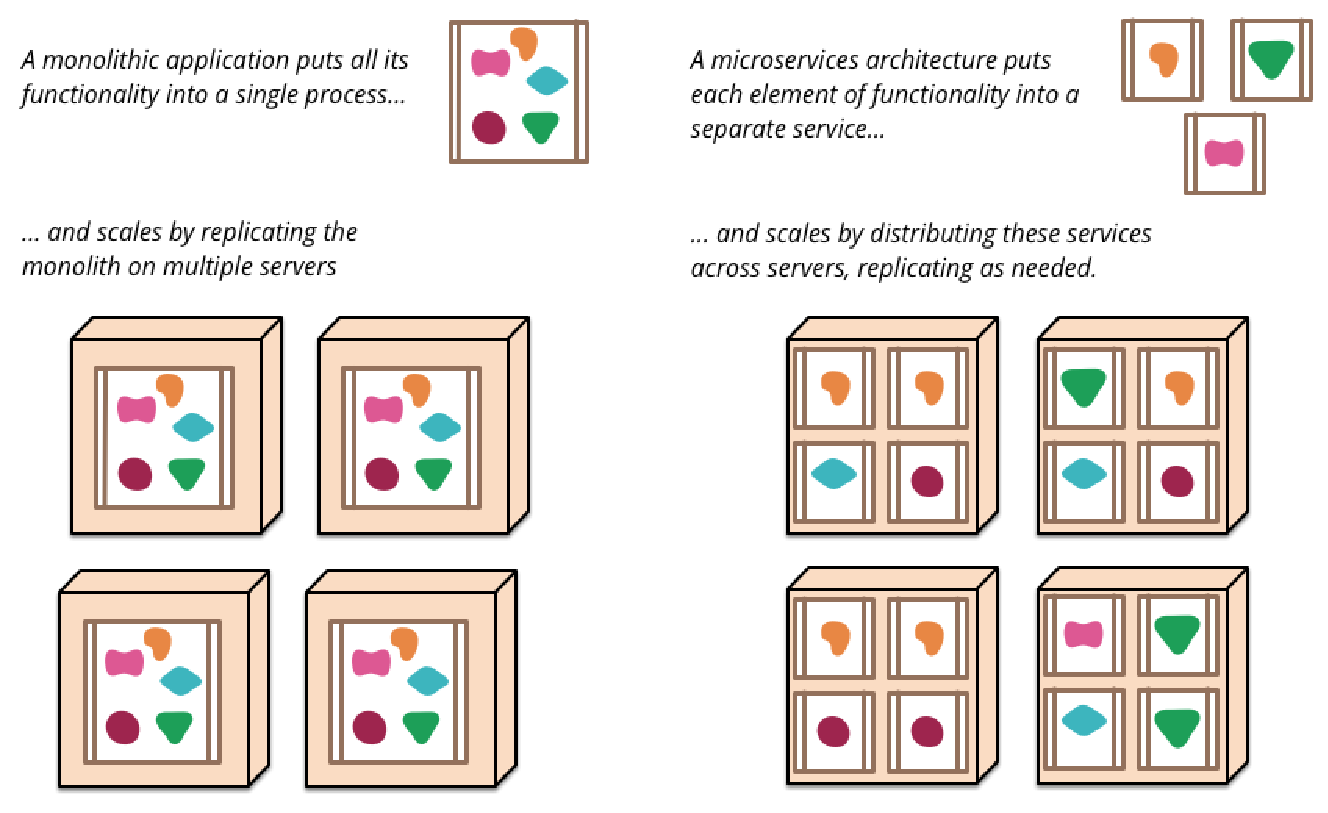
\includegraphics[width=1.00\textwidth]{monolithic_and_microservices.pdf}
    \caption{Monolithic and Microservices architectural styles~\cite{microservices}.}
    \label{fig:monolithic_and_microservices}
\end{figure}

Both styles presented have their own advantages and disadvantages. To briefly present some of them, two examples are provided, one for each architectural style. First example: if one team needs to develop a single process system, e.g., e-Commerce application, that authorizes customer, takes an order, check products inventory, authorize payment and ships ordered products. The best alternative is to use Monolithic architecture, because they can develop every feature in a single software package due to the application simplicity, however, if the client starts to demand hard changes and additional features in the solution, the code base may tend to increase into ``out of control'', leading to more challenging and time consuming changes. Second example, if one team needs to develop a complex and huge service that needs to scale, e.g., Video streaming service, the best alternative is to use Microservices architecture, because they can tackle the problem of complexity by decomposing the application into a set of manageable small services which are much faster to develop and test by individual organized teams, and thus, it will be easier to maintain the code base due to decoupling, however, it will be harder to monitor and manage the entire platform due to additional complexity associated with distributed systems.

Taking into consideration this increasing difficulty in monitoring and managing large Microservice based platforms, one must be aware and observe system behaviour to be able to control it. Therefore, in the next Subsection~\ref{subsec:observability_and_controlling_performance}, the core concept of~\nameref{subsec:observability_and_controlling_performance} is explained.

\subsection{Observability and Controlling Performance}
\label{subsec:observability_and_controlling_performance}

This Subsection aims to provide an introduction to some theory concepts about Observability and Performance Controlling, regarding distributed software systems.

Observability is a meaningfully extension of the word observing. Observing is ``to be or become aware of, especially through careful and directed attention; to notice'~'\cite{observing_definition}. The term Observability comes from the world of engineering and control theory. Observability is not a new term in the industry, however it has gain more focus in the last years due to \gls{devops} raising. It means by definition ``to measure of how well internal states of a system can be inferred from knowledge of its external outputs''~\cite{observability}. Therefore, if our good old software systems and applications do not adequately externalize their state, then even the best monitoring can fall short.

Controlling in control systems is ``to manage the behaviour of a certain system''~\cite{control_systems}. Controlling and Observability are dual aspects of the same problem~\cite{observability}, as we need to have information to infer state and be able take action. E.g., When observing an exponential increase in the \gls{cpu} load, the system scales horizontally invoking more machines and spreading the work between them to easy handle the work. This is a clear and simple example that conjugates the terms presented, we have: values that are observed ``Observability'' and action that leads to system control ``Controlling Performance''.

When we want to understand the working and behaviour of a system, we need to watch it very closely and pay special attention to all details and information it provides. Microservice based systems produce multiple types of information if instrumented. These type of information are the ones mentioned in Chapter~\ref{chap:introduction}: Monitoring, Tracing and Logging. In this thesis, the goal is to use tracing data thus, this type of produced information is the one to focus.

In the next Subsection~\ref{subsec:distributed_tracing}~-~\nameref{subsec:distributed_tracing}, the type of data mentioned before is presented and explained in detail.

\subsection{Distributed Tracing}
\label{subsec:distributed_tracing}

%\todo{How to introduce Google Dapper~\cite{Sigelman2010}}

Distributed tracing~\cite{Sambasivan2016} is a method that comes from traditional tracing, but applied to a distributed system at the work-flow level. It profiles and monitor applications, especially those built using microservice architectures and, in the end, it can be used to help DevOps teams pinpoint where failures occur and why.

A number of tools and standards emerged from this concept. For example, the OpenTracing standard~\cite{open_tracing_data_model_specification} follows the model proposed by Fonseca~\textit{et al.}~\cite{fonseca2007x}, which defines traces as a tree of spans representing scopes or units of work (i.e., thread, function, service). These traces enable following such units of work through the system.

OpenTracing uses dynamic, fixed-width metadata to propagate causality between spans, meaning that each span has a \emph{trace identifier} common to all spans of the same trace, as well as a \emph{span identifier} and \emph{parent identifier} representing parent/child relationships between spans~\cite{Sambasivan2014}. The standard defines the format for spans and the semantic~\cite{open_tracing_semantic_specification, open_tracing_semantic_conventions} conventions for their content/annotations.

%Usually, the span has an operation name, the start time of the operation, its duration and some annotations regarding the operation itself. An example of a span can be an HTTP call or a Remote Procedure Call (RPC). 

Figure~\ref{fig:sample_trace_over_time} provides a clear insight about how spans are related to time and with each other.

\begin{figure}[H]
    \centerline{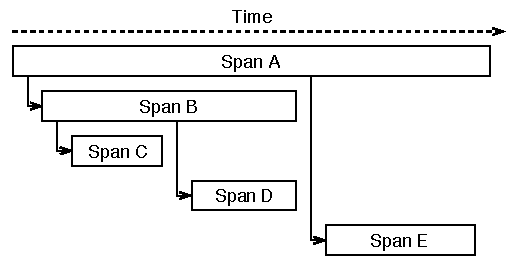
\includegraphics[width=1.0\linewidth]{images/trace.pdf}}
    \caption{Sample trace over time.}
    \label{fig:sample_trace_over_time}
\end{figure}

In Figure~\ref{fig:sample_trace_over_time} there are a group of five spans spread through time that represents a trace. A trace is a group of spans that share the same \emph{TraceID}.  A trace is a representation of a data/execution path in the system. A span represents the logical unit of work in the system. A trace can also be a span, if there is only one span presented in the trace. One span can cause another.

Causality relationship between spans can be observed in Figure~\ref{fig:sample_trace_over_time}, where ``Span A'' causes ``Span B'' and ``Span E'', moreover, ``Span B'' causes ``Span C'' and ``Span D''. From this we say that ``Span A'' is parent of ``Span B'' and ``Span E''. Likewise, ``Span B'' and ``Span E'' are children of ``Span A''. In this case, ``Span A'' does not have a parent, it is an ``orphan span'' and therefore, is the root span and the origin of this whole trace. Spans carry with them metadata like e.g., \emph{SpanID} and \emph{ParentID}, that allows to infer this relationships.

Disposition of spans over time is another clear fact that can be observed from the representation in Figure~\ref{fig:sample_trace_over_time}. Spans have a begin and an end in time. This causes them to have a duration. Spans are spread through time, however they usually stay inside parent boundaries, this means that the duration of a parent span always covers durations of their children. Considering a parent and a child spans, if they are related, the parent span always start before child span, also, the parent span always end after child span. Note that nothing prevents multiple spans to start in the same exact moment. Span also carry with them metadata like e.g., \emph{Timestamp} and \emph{Duration}, that allows to infer their position in time and when they end.

An example of a span can be an \gls{http} call or a \gls{rpc} call. We may think of the following cases to define each operation inherent to each box presented in Figure~\ref{fig:sample_trace_over_time}: A - ``Get user info'', B - ``Fetch user data from database'', C - ``Connect to MySQL server'', D - ``Can't connect to MySQL server'' and E - ``Send error result to client''.

In the data model specification, the creators of OpenTracing say that: ``with a couple of spans, we might be able to generate a span tree and model a directed graph of a portion of the system''~\cite{open_tracing_data_model_specification}. This is due to the causal relationships they represent. Apart from the root span every other span must have a parent. Figure~\ref{fig:span_tree_example} provides an example of a span tree.

\begin{figure}[H]
    \centering
    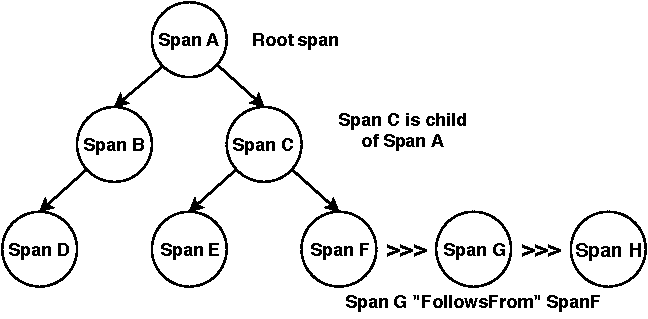
\includegraphics[width=1.0\linewidth]{span_tree_example.pdf}
    \caption{Span Tree example.}
    \label{fig:span_tree_example}
\end{figure}

Figure~\ref{fig:span_tree_example} contains a span tree representation with a trace containing eight spans. As said before,every span must be a child of some other span, unless it is the root span, this is very clear in a span tree visualization with the usage of the root node. With this causal relationship, a path through the system can be retrieved. For example, if for example every span processes in a different endpoint represented by letters presented in the span tree, one may generate the request path: A ---$>$ B ---$>$ D. This means that our hypothetical request passed through machine A, B and D, or if it were services, the request passed from service A, to B and finally to D. From this, we can generate the dependency graph of the system (explained in the Subsection~\ref{subsec:graphs}~-~\nameref{subsec:graphs}).

This type of data is extracted as trace files or streamed over transfer protocols like e.g., \gls{http}, from technologies like Kubernetes~\cite{what_is_kubernetes}, OpenStack~\cite{what_is_opensatck}, and other cloud or distributed management system technologies that implements some kind of system or code instrumentation using, for example, OpenTracing~\cite{what_is_opentracing} or OpenCensus~\cite{what_is_opencensus}. Tracing contains some vital system details as they are the result of system instrumentation and therefore, this data can be used as a resource to provide observability over the distributed system.

As said before, from the causality relationship between spans we can generate a dependency graph of the system. The next Subsection~\ref{subsec:graphs}~-~\nameref{subsec:graphs} aims to provide a clear understand of this concept and how they relate with distributed tracing.

\subsection{Graphs}
\label{subsec:graphs}

From distributed tracing we can be able to extract the system dependency graph from a representative set of traces. To introduce the concept of Graph, ``A Graph is a set of vertices and a collection of directed edges that each connects an ordered pair of vertices''~\cite{graph_standard_definition}.

Taking the very common sense of the term and to provide notation, a graph, $G$, is an ordered pair $G = (V, E)$, where $V$ are the vertices/nodes and $E$ are the edges.

Graphs are defined by:

\begin{itemize}
    \item Node: Are the entities in the graph. They can hold any number of attributes (key-value pairs) called properties. Nodes can be tagged with labels, representing their different roles in a domain. Node labels may also serve to attach metadata (such as index or constraint information) to certain nodes;
    \item Edge (or Relationships): provide directed, named, semantically-relevant connections between two node entities;
    \item Property: can be any kind of metadata attached to a certain Node or a certain Edge.
\end{itemize}

Also, there are multiple types of graphs, they can be:

\begin{enumerate}
    \item Undirected-Graph: the set of edges without orientation between a pair of nodes;
    \item Directed-Graph: the set of edges have one and only one direction between a pair of nodes;
    \item Multi-Directed-Graph: multiple edges have more than one connection between a pair of nodes that represents the same relationship.
\end{enumerate}

Figure~\ref{fig:graphs_types} gives us a simple visual representation of what a graph really is for a more clear understanding.

\begin{figure}[H]
    \centering
    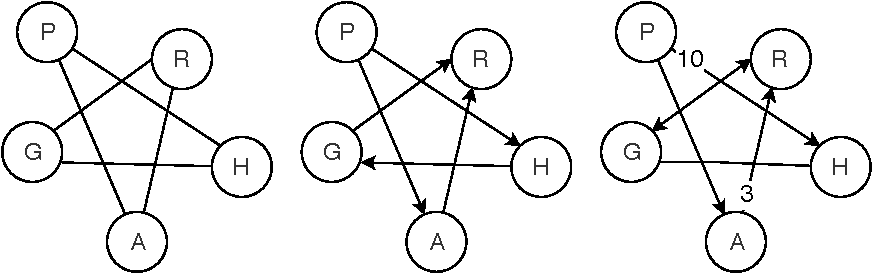
\includegraphics[width=1.00\textwidth]{images/graph_representations.pdf}
    \caption{Graphs types.}
    \label{fig:graphs_types}
\end{figure}

In Figure~\ref{fig:graphs_types} three identical graphs are presented and each one is composed by five nodes, however, they are not equal because each one has it own type. They belong respectively to each type enumerated above. From left to right, the first graph is a Undirected-Graph, the second one is a Directed-Graph and the last one is a Multi-Directed-Graph.

The last graph has some numbers in some edges. Every graph can have this annotations. These can provide some information about the connection between the pair of nodes. For example, in distributed systems context, if this graph represents our system dependency graph, and nodes $H$ and $P$ hypothetical services, the edge between them could represent calls between these two service and the notation number the number of calls with respect to the edge direction. Therefore, in this case, we would have 10 requests from incoming from $P$ to $H$.

Figure~\ref{fig:service_dependency_graph} provides a clear insight about service dependency graphs.

\begin{figure}[H]
    \centering
    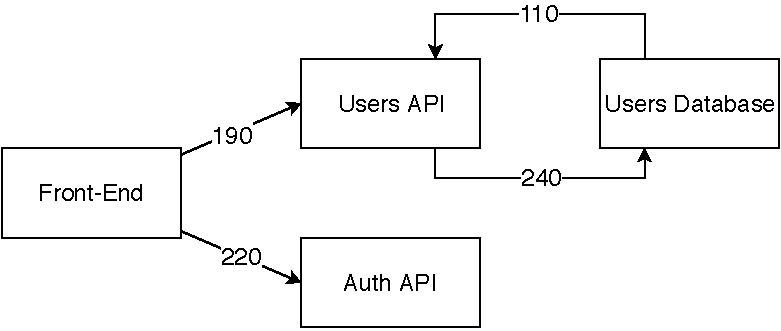
\includegraphics[width=1.00\textwidth]{images/graph_service_representation.pdf}
    \caption{Service dependency graph.}
    \label{fig:service_dependency_graph}
\end{figure}

In Figure~\ref{fig:service_dependency_graph}, a representation of a service dependency graph is provided. Service dependency graphs are graphs of type Multi-Directed-Graph, because they have multiple edges with more than one direction between a pair of services(Nodes). In this representation, there are multiple services involved, each inside a box. The edges between boxes (Nodes), indicate the number of calls that each pair of services invoked, e.g., ``Users API'' called ``Users Database'' 240 times. These dependency graphs gives the state of the system in a given time interval. This can be useful to study the changes in the morphology of the system, e.g., a service disappeared and a set of new ones appeared. Other interesting study could be the variation in the amount of call between services.

Graphs are a way to model and extract information from tracing data. Another interesting approach could be to extract metrics in time from tracing because traces and spans are spread in time, and they have information about the state of the system at a given instant. The next Subsection~\ref{subsec:time_series}~-~\nameref{subsec:time_series} provides an introduction to a data representation model.

\subsection{Time Series}
\label{subsec:time_series}

Time-Series are a way of representing data as a time-indexed series of values. This kind of data is often arise when monitoring systems, industrial processes, tracking corporate business metrics or sensor measurements. Figure~\ref{fig:time_series_example} provides a visual example of this way of data representation.

\begin{figure}[H]
    \centering
    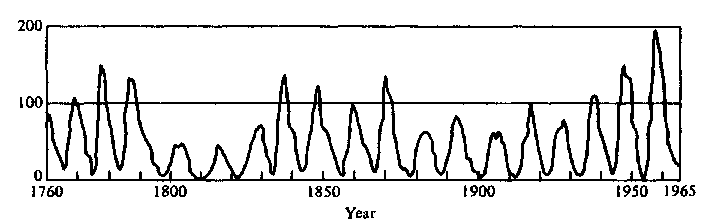
\includegraphics[width=1.00\textwidth]{images/time_series_example.pdf}
    \caption{Time series: Annual mean sunspot numbers for 1760-1965~\cite{Brillinger2006}.}
    \label{fig:time_series_example}
\end{figure}

In Figure~\ref{fig:time_series_example}, Brillinger \textit{D.}~\cite{Brillinger2006} presents a visual representation of a time-series as a collection of values in time. These values are measurements of sunspot means gathered from 1960-1965. In this case, measurements come from natural origin, however, one can perform observations of e.g., \gls{cpu} load, system uptime / downtime and network latency.

As these processes are not random, autocorrelation can be exploited to extract insight from the data, such as predict patterns or detect anomalies. Therefore, time-series data can be analysed to detect anomalies present in the system. One way to do this is to look for outliers~\cite{Liu2004} in the multidimensional feature set. Anomaly detection in time series data is a data mining process used to determine types of anomalies found in a data set and to determine details about their occurrences. Anomaly detection methods are particularly interesting for our data set since it would be impossible to manually tag the set of interesting anomalous points. Figure~\ref{fig:time_series_anomaly_detection_example} provides a simple visual representation of anomaly detection in time series data.

\begin{figure}[H]
    \centering
    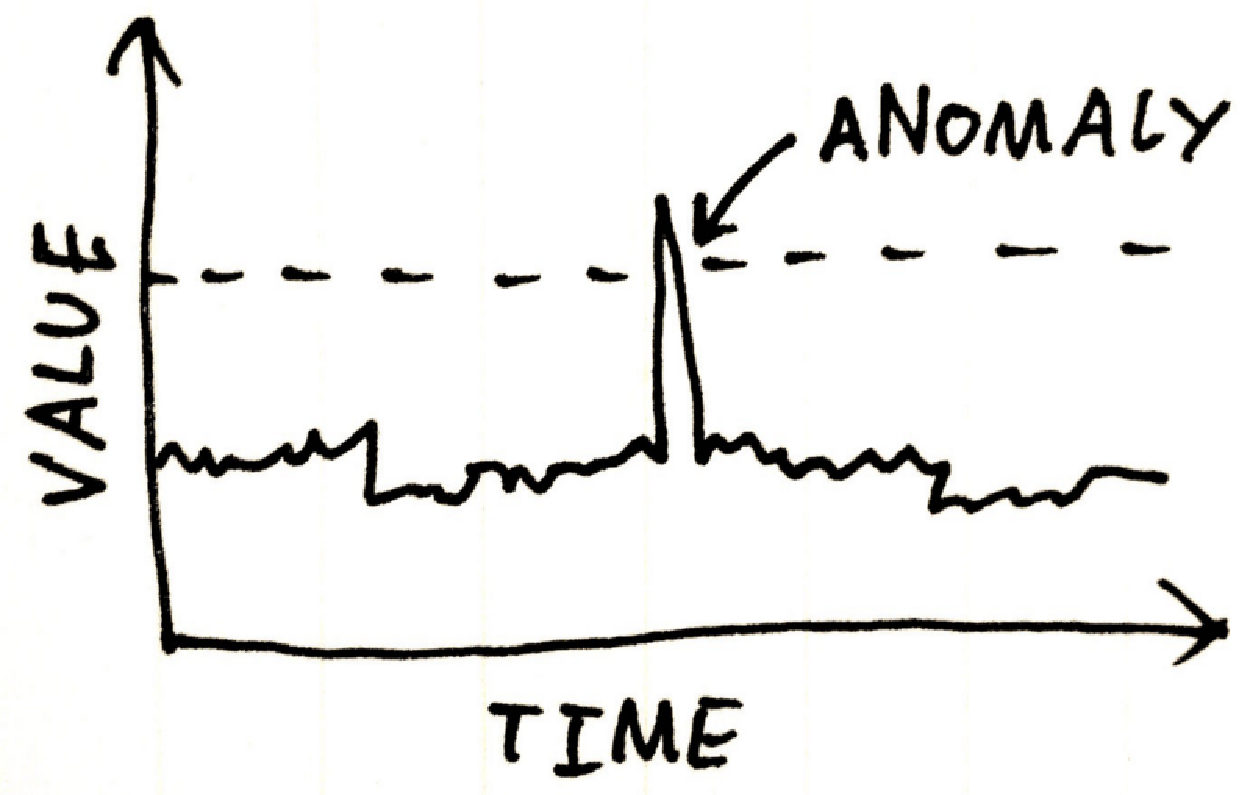
\includegraphics[width=0.50\textwidth]{images/time_series_anomaly_detection_example.pdf}
    \caption{Anomaly detection in Time Series~\cite{NikolajBomannMertz}.}
    \label{fig:time_series_anomaly_detection_example}
\end{figure}

In Figure~\ref{fig:time_series_anomaly_detection_example}, there is a clear spike in values from this time series measurements. This can be declared an outlier because it is a strange value considering the range of remaining measurements and therefore, it is considered an anomaly. In this example, anomaly detection is easy to perform by a Human, however, in mostly cases nowadays, due to great variation of values and plethora of information that can be gathered, perform this detection manually is impracticable, thus automatic anomaly detection using Machine Learning techniques are used nowadays.

Anomaly detection in time series data is a data mining process used to determine types of anomalies found in a data set and to determine details about their occurrences. This auto anomaly detection method has lots of usage due to the impossible work of tag manually the interesting set of anomalous points. Auto anomaly detection has a wide range of applications such as fraud detection, system health monitoring, fault detection, event detection systems in sensor networks, and so on.

After explaining the core concepts, foundations for the work presented in this thesis, to the reader, technologies capable of handling this types of information are presented and discussed in next Section~\ref{sec:technologies}~-~\nameref{sec:technologies}.

\section{Technologies}
\label{sec:technologies}

In this section are presented technologies and tools capable of handling the types of information discussed in the previous Section~\ref{sec:concepts}~-~\nameref{sec:concepts}.

The main tools covered are:~\ref{subsec:distributed_tracing_tools}~-~\nameref{subsec:distributed_tracing_tools}, for distributed tracing data handling, \ref{subsec:graph_manipulation_and_processing_tools}~-~\nameref{subsec:graph_manipulation_and_processing_tools} and~\ref{subsec:graph_database_tools}~-~\nameref{subsec:graph_database_tools}, for graph processing and storage, and~\ref{subsec:time_series_database_tools}~-~\nameref{subsec:time_series_database_tools}, for time series value storage.

\subsection{Distributed Tracing Tools}
\label{subsec:distributed_tracing_tools}

This Subsection presents the most used and known distributed tracing tools. These tools are mainly oriented for tracing distributed systems like microservices-based applications. What they do is to fetch or receive trace data from this kind of complex systems, treat the information, and then present it to the user using charts and diagrams in order to explore the data in a more human-readable way. One of the best features presented in this tools, is the possibility to perform queries on the tracing (e.g., by trace id and by time-frame). Table~\ref{table:distributed_tracing_tools} presents the most well-known open source tracing tools.

\begin{table}[]
    \caption{Distributed tracing tools comparison.}
    \label{table:distributed_tracing_tools}
    \centering
    \begin{tabularx}{\linewidth} {
            >{\hsize=0.234\hsize}X|
            >{\hsize=0,383\hsize}X|
            >{\hsize=0,383\hsize}X|}
        \cline{2-3}

         & Jaeger~\cite{Jaeger}
         & Zipkin~\cite{Zipkin}                                                                                                                                                                                  \\ \hline \hline
        \multicolumn{1}{|l|}{\textbf{Brief description}}
         & Released as open source by Uber Technologies. Used for monitoring and troubleshooting microservices-based distributed systems. Was inspired by Zipkin.
         & Helps gathering timing data needed to troubleshoot latency problems in microservice applications. It manages both the collection and lookup of this data. Zipkin's design is based on the Google Dapper paper. \\ \hline
        \multicolumn{1}{|l|}{\textbf{Pros}}
         & Open source; \newline
        Docker-ready; \newline
        Collector interface is compatible with Zipkin protocol; \newline
        Dynamic sampling rate; \newline
        Browser user interface.
         & Open source; \newline
        Docker-ready; \newline
        Allows multiple span transport technologies (HTTP, Kafka, Scribe, AMQP); \newline
        Browser user interface.                                                                                                                                                                                                     \\ \hline
        \multicolumn{1}{|l|}{\textbf{Cons}}
         & Only supports two span transport ways (Thrift and HTTP).
         & Fixed sampling rate.                                                                                                                                                                                         \\ \hline
        \multicolumn{1}{|l|}{\textbf{Analysis}}
         & Dependency graph view; \newline
        Trace comparison (End 2018).
         & Dependency graph view.                                                                                                                                                                                       \\ \hline
        \multicolumn{1}{|l|}{\textbf{Used by}}
         & Red Hat; \newline
        Symantec; \newline
        Uber. \newline
         & AirBnb; \newline
        IBM; \newline
        Lightstep.                                                                                                                                                                                                      \\ \hline
    \end{tabularx}
\end{table}

In Table~\ref{table:distributed_tracing_tools}, we can see that these two tools are very similar. Both are open source projects, allow docker containerization and provide a browser ui to simplify user interaction. Jaeger was created by Uber and the design was based on Zipkin, however, it does not provide much more features. The best feature that was released for Jaeger in the past year was the capability of perform trace comparison, where the user can select a pair of traces and compare them in terms of structure. This is a good effort in additional features, but it is short in versatility because we can only compare a pair of traces in a ``sea'' of thousands, or even millions.

These tools aim to collect trace information and provide a user interface with some query capabilities for \gls{devops} to use. However they are always focused on span and trace lookup and presentation, and do not provide a more interesting analysis of the system, for example to determine if there is any problem related to some microservice presented in the system. This kind of work falls into the user, \gls{devops}, as they need to perform the tedious work of investigation and analyse the tracing with the objective of find anything wrong with them.

This kind of tools can be a good starting point for the problem that we face, because they already do some work for us like grouping the data generated by the system and provide a good representation for them.

In next Subsection~\ref{subsec:graph_manipulation_and_processing_tools}, graph manipulation and processing tools are presented and discussed.

\subsection{Graph Manipulation and Processing Tools}
\label{subsec:graph_manipulation_and_processing_tools}

Distributed tracing is a type of data produced by Microservice based architectures. This type of data is composed by traces and spans. With a set of related spans, a service dependency graph can be produced. This dependency graph is a Multi-Directed-Graph, as presented in Subsection~\ref{subsec:graphs}. Therefore, with this data at our disposal, there is the need of a graph manipulation and processing tool.

In this Subsection, the state of the art about graph manipulation and processing tools is presented. Graphs are non-linear data structure representations consisting of nodes and edges. Nodes are sometimes also referred to as vertices and edges are lines or arcs that connect any pair of nodes in the graph. This data structure takes some particular approaches when handling their contents, because there are some special attributes related. For example, perform the calculation of the degree of some node -- degree of a node is the number of edges that connect to the node itself; Calculate how many nodes entered and exited the graph by comparing it to another one; Know the difference in edges between two distinct graphs~\cite{Trudeau1993}.

Taking into consideration this data structure, the particularities involved and the need to use graphs to manipulate service dependencies, frameworks with features capable of handling and retrieving graphs are a need. Therefore, Table~\ref{table:graph_manipulation_and_processing_tools_comparison} presents a comparison of the main tools available at the time for graph manipulation and processing.

\begin{table}[H]
    \caption{Graph manipulation and processing tools comparison.}
    \label{table:graph_manipulation_and_processing_tools_comparison}
    \centering
    \begin{tabularx}{\linewidth} {
            >{\hsize=0.3\hsize}X|
            >{\hsize=1.0\hsize}X|
            >{\hsize=1.0\hsize}X|
            >{\hsize=1.0\hsize}X|}
        \cline{2-4}

         & Apache Giraph \cite{apache_giraph}
         & Ligra \cite{ligra_graph_processing_framework}
         & NetworkX \cite{networkx}                                                                                                                                                       \\ \hline \hline
        \multicolumn{1}{|l|}{\textbf{Description}}
         & An iterative graph processing system built for high scalability. Currently used at Facebook to analyse the social graph formed by users and their relationships.
         & A library collection for graph creation, analysis and manipulation of networks.
         & A Python package for the creation, manipulation, and study of structure, dynamics, and functions of complex networks.                                                          \\ \hline
        \multicolumn{1}{|l|}{\textbf{Licence}~\cite{Morin2012}}
         & Free Apache 2.
         & MIT.
         & BSD - New License.                                                                                                                                                             \\ \hline
        \multicolumn{1}{|p{2.2cm}|}{\textbf{Supported languages}}
         & Java and Scala.
         & C and C++.
         & Python.                                                                                                                                                                        \\ \hline
        \multicolumn{1}{|l|}{\textbf{Pros}}
         & Distributed and very scalable; \newline
        Excellent performance -- Process one trillion edges using 200 modest machines in 4 minutes.
         & Handles very large graphs; \newline
        Exploit large memory and multi-core \gls{cpu} -- Vertically scalable.
         & Good support and very easy to install with Python; \newline
        Lots of graph algorithms already implemented and tested. \newline                                                                                                                 \\ \hline
        \multicolumn{1}{|l|}{\textbf{Cons}}
         & Uses ``Think-Like-a-Vertex'' programming model that often forces into using sub-optimal algorithms, thus is quite limited and sacrifices performance for scaling out; \newline
        Unable to perform many complex graph analysis tasks because it primarily supports Bulk synchronous parallel.
         & Lack of documentation and therefore, very hard to use; \newline
        Does not have many usage in the community.
         & Not scalable (single-machine); \newline
        High learning curve due to the maturity of the project; \newline
        Begins to slow down when processing high amount of data -- 400.000+ nodes.                                                                                                        \\ \hline
    \end{tabularx}
\end{table}

Table~\ref{table:graph_manipulation_and_processing_tools_comparison} presents some key points to consider when choosing a graph manipulation and processing tool.

First, one aspect to be considered when comparing them is the scalability and performance that each provide. Apache Giraph is the best tool in this field, since it is implemented with distributed and parallel computation, which allows it to scale to multiple-machines, sharing the load between them, and processing data large quantities of data in less time than the remaining presented tools. On the opposite side, NetworkX, only works in a single-machine environment which does not allow it scale to multiple-machines. Ligra, like the previous tool, works in a single-machine environment, however it benefits from vertical scale on a single-machine, which allows to exploit multi-core \gls{cpu} and large memory. NetworkX and Ligra are tools that can present a bottleneck in a system where the main focus is to handle large amounts of data in short times.

\,

Secondly, another aspect to be considered is the support and quantity of implemented graph algorithms available on the frameworks. NetworkX have advantages in this aspect, because it contains implementation of the majority graph algorithms defined and studied in graph and networking theory. Also, due to project maturity, it has a good documentation support from the community who keeps all the information updated. Ligra framework has lack of documentation, which causes tremendous difficulty for developers to use and know what are the implemented features. Apache Giraph, does not support a large set of graph processing algorithms due to implementation constraints.

Figure~\ref{fig:graph_tools_comparison} gives a clear insight when comparing these tools from two features -- scalability / performance against implementation of graph algorithms.

\begin{figure}[H]
    \centering
    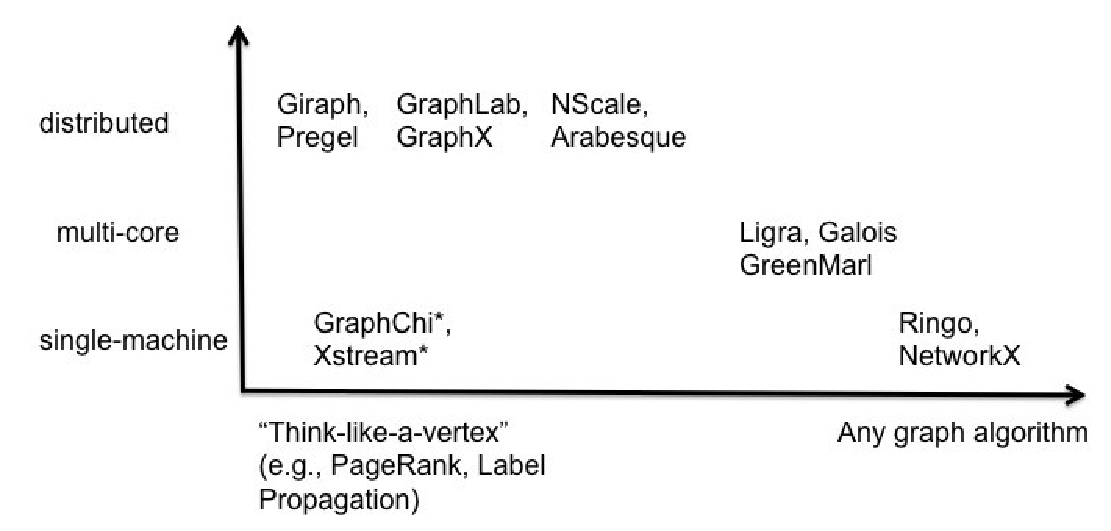
\includegraphics[width=1.0\linewidth]{images/graph_manipulation_tools_diagram_comparison.pdf}
    \caption{Graph tools: Scalability vs. Algorithm implementation~\cite{graph_data_management_systems}.}
    \label{fig:graph_tools_comparison}
\end{figure}

In Figure~\ref{fig:graph_tools_comparison} we can observe tools disposition regarding the two aspect key points explained before. This figure contains all tools presented over two featured axis: one for scalability and the other for implementation of graph algorithms. Tools placement in this chart proves and reinforces the comparison presented before. Apache Giraph and NetworkX are placed in the edges of these features, which means that Apache Giraph can be found in the upper left region of the chart -- highly distributed but minimally in graph algorithms implementation --, and NetworkX is in the lower right region -- minimally distributed but highly in graph algorithms implementation.

After discussing tools capable of manipulate and process graphs, their storage is a need for later usage. \gls{gdb} storage technologies are presented in next Subsection~\ref{subsec:graph_database_tools}~-~\nameref{subsec:graph_database_tools}.

\subsection{Graph Database Tools}
\label{subsec:graph_database_tools}

Graph databases represent a way of persisting graph information. After having instantiated a Graph, processed it in volatile memory, they can be stored in persistent memory for later use. To do this one can use a \gls{gdb}. A \gls{gdb} is ``a database that allows graph data storing and uses graph structures for semantic queries with nodes, edges and properties to represent them''~\cite{Celko2013}.

\newpage

Based upon the concept of a mathematical graph, a graph database contains a collection of nodes and edges. A node represents an object, and an edge represents the connection or relationship between two objects. Each node in a graph database is identified by a unique identifier that expresses key value pairs. Additionally, each edge is defined by a unique identifier that details a starting or ending node, along with a set of properties. Graph databases are becoming popular due to Machine Learning and Artificial Intelligence grows, since a number of Machine Learning algorithms are inherently graph algorithms~\cite{FavioVazquez2019}.

Furthermore, in this research service dependency graphs are highly used, thus the need to use a \gls{gdb}. Table~\ref{table:graph_databases_comparison} contains the most well-known \gls{gdb}.

\begin{table}[H]
    \caption{Graph databases comparison.}
    \label{table:graph_databases_comparison}
    \centering
    \begin{tabularx}{\linewidth} {
            >{\hsize=0.3\hsize}X|
            >{\hsize=1.0\hsize}X|
            >{\hsize=1.0\hsize}X|
            >{\hsize=1.0\hsize}X|}
        \cline{2-4}

         & ArangoDB \cite{arangodb_documentation}
         & Facebook TAO \cite{Amenya2018}
         & Neo4J \cite{neo4j_documentation}                                                                                               \\ \hline \hline
        \multicolumn{1}{|l|}{\textbf{Description}}
         & A NoSQL database that uses a proper query language to access the database.
         & TAO, “The Associations and Objects”, is a proprietary graph database, developed by Facebook, used to store the social network.
         & The most popular open source graph database, completely open to the community.                                                 \\ \hline
        \multicolumn{1}{|l|}{\textbf{Licence}~\cite{Morin2012}}
         & Free Apache 2.
         & Proprietary.
         & GPLv3 CE.                                                                                                                      \\ \hline
        \multicolumn{1}{|p{2.2cm}|}{\textbf{Supported} \newline \textbf{languages}}
         & C++; Go; Java; JavaScript; Python and Scala.
         & Go; Java; JavaScript; Python and Scala.
         & Java; JavaScript; Python and Scala.                                                                                            \\ \hline
        \multicolumn{1}{|l|}{\textbf{Pros}}
         & Multi data-type support (key/value, documents and graphs); \newline
        Allows combination of different data access patterns in a single query; \newline
        Supports cluster deployment.
         & Low latency $(~=100ms)$; \newline
        Accepts millions of calls per second; \newline
        Distributed database.
         & Supports ACID(Atomicity, Consistency, Isolation, Durability)~\cite{Sasaki2018}; \newline
        Most popular open source graph database.                                                                                          \\ \hline
        \multicolumn{1}{|l|}{\textbf{Cons}}
         & High learning curve due to AQL (Arango Query Language); \newline
        Has paid version with high price tag.
         & Not accessible to use.
         & Not able to scale horizontally.                                                                                                \\ \hline
    \end{tabularx}
\end{table}

From Table~\ref{table:graph_databases_comparison} we can notice that the state of the art for \gls{gdb} is not very pleasant. Interest for this type of databases has began in the later years due to artificial intelligence and machine learning trends, therefore, the offer presented in the field are limited.

Back in time, when social network tendency emerged, the development of this type of databases raised, and the most powerful technologies for graph storage where developed in closed source. One example is \emph{Facebook TAO} database presented in Table~\ref{table:graph_databases_comparison}, a database developed by the company to support the entire social network, storing users in nodes and their relationships in edges. This database is described by having very low latency, which stands for high response time, however, very few information regarding this tool can be found -- just some scientific papers~\cite{facebook_tao_article,Facebook2150}.
% only few scientific papers were found

The remaining tools presented are available for usage. ArangoDB has multi data-type support, which means that a wider type of data structures are supported for storing in nodes and edges metadata. Also, it supports scalability through cluster deployment, however, this feature is only available in paid versions -- Arango SmartGraphs storage improves the writing of graph in distributed systems environment~\cite{arangodb_smart_graphs}. The biggest disadvantage of this database is the high learning curve associated with the usage of \emph{AQL (Arango Query Language)}, however, this disadvantage can be surpassed by using provided \gls{api} clients with the trade-off of loosing some control.

\emph{Neo4J} is the most accepted \gls{gdb} by the open source community. This \gls{gdb} has increased in popularity in the past years due to simplicity and easy support~\cite{Turu2017}. Trade-offs from this database consists in lack of support for scalability, which means that this database can only run on a single-machine environment, however, there are some users reporting that they were able to perform implementations and surpass the lack of support for horizontal scaling, but this is not tested~\cite{neo4j_scalable}.

Choosing a graph database can be hard because these tools are growing and the tendency for changes in features and tooling support is very high, however,  the decision falls on the question of easy of usage and horizontal scalability. This means that \emph{ArangoDB} is a database more advised for big projects, where the size of graphs to store may surpass the limit of a single-machine, and Neo4J for simpler projects, where the focus are functionality testing and prototyping, and graph storage represents a side concern.

Next Subsection~\ref{subsec:time_series_database_tools}~-~\nameref{subsec:time_series_database_tools} covers the state of the art for tooling capable of storage values based in time.

\subsection{Time-Series Database Tools}
\label{subsec:time_series_database_tools}

In this Subsection, tools for storing time-indexed series of values are presented. This type of data is a need for this research due to the tight relation between distributed tracing and time, as explained in Subsections~\ref{subsec:distributed_tracing} and~\ref{subsec:time_series}. Also, service dependency graphs, as a representation of the system at a given time, can contain valuable information for monitoring Microservice systems. For this purpose, \gls{tsdb} are databases capable of storing time-series based values.

A \gls{tsdb} is ``A database optimised for time-stamped or time series data like arrays of numbers indexed by time (a date time or a date time range)''~\cite{Dunning2015}. These databases are natively implemented using specialised time-series theory algorithms to enhance their performance and efficiency, due to widely variance of access possible. The way this databases use to work on efficiency is to treat time as a discrete quantity rather than as a continuous mathematical dimension. Usually a \gls{tsdb} allows operations like create, enumerate, update, organise and destroy various time series entries in short access times.

This type of database is growing in usage and popularity because of Internet of Things (IoT) trend. Discussions in this area have increased over the past few years, and is expected that it keeps increasing, due to Ubiquitous Computing -- Raise of omnipresent and universal technologies. At the same time, \gls{tsdb} grows with this IoT tendency, because data mining from sensor spread geographically and sensors gather information through measurements in specific points in time. This information are usually stored in \gls{tsdb}~\cite{TanayPant2019}.

\newpage

Table~\ref{table:time_series_databases_comparison} presents a comparison between two \gls{tsdb}: \textit{InfluxDb} and \textit{OpenTSDB}.

\begin{table}[H]
    \caption{Time-series databases comparison.}
    \label{table:time_series_databases_comparison}
    \centering
    \begin{tabularx}{\linewidth} {
            >{\hsize=0.60\hsize}X|
            >{\hsize=1.20\hsize}X|
            >{\hsize=1.20\hsize}X|}
        \cline{2-3}

         & InfluxDB \cite{influxdb}
         & OpenTSDB \cite{opentsdb}                                                                                                                                                                                                                                       \\ \hline \hline
        \multicolumn{1}{|l|}{\textbf{Description}}
         & An open-source time series database written in Go and optimised for fast, high-availability storage and retrieval of time series data in fields such as operations monitoring, application metrics, Internet of Things sensor data, and real-time analytics's.
         & A distributed and scalable \gls{tsdb} written on top of HBase; \newline
        OpenTSDB was written to address a common need: store, index and serve metrics collected from computer systems (network gear, operating systems and applications) at a large scale, therefore, making this data easily accessible and displayed.                   \\ \hline
        \multicolumn{1}{|l|}{\textbf{Licence}~\cite{Morin2012}}
         & MIT.
         & GPL.                                                                                                                                                                                                                                                           \\ \hline
        \multicolumn{1}{|p{2.2cm}|}{\textbf{Supported languages}}
         & Erlang, Go, Java, JavaScript, Lisp, Python, R and Scala.
         & Erlang, Go, Java, Python, R and Ruby.                                                                                                                                                                                                                          \\ \hline
        \multicolumn{1}{|l|}{\textbf{Pros}}
         & Scalable in the enterprise version; \newline
        Outstanding high performance; \newline
        Accepts data from \gls{http}, TCP, and UDP protocols; \newline
        SQL like query language; \newline
        Allows real-time analytics's.
         & Massively scalable; \newline
        Great for large amounts of time-based events or logs; \newline
        Accepts data from \gls{http} and TCP protocols; \newline
        Good platform for future analytical research into particular aggregations on event / log data; \newline
        Does not have paid version.                                                                                                                                                                                                                                       \\ \hline
        \multicolumn{1}{|l|}{\textbf{Cons}}
         & Enterprise high price tag; \newline
        Clustering support only available in the enterprise version.
         & Hard to set up; \newline
        Not a good choice for general-purpose application data.                                                                                                                                                                                                           \\ \hline
    \end{tabularx}
\end{table}

From Table~\ref{table:time_series_databases_comparison}, we can notice some similarities between these two \gls{tsdb} databases. Both \gls{tsdb} are capable scalable and accept \gls{http} and TCP transfer protocols for communication. InfluxDB and OpenTSDB are two open source time-series databases, however, the first one, InfluxDB, is not completely free, as it has an enterprise paid version, which is not very visible in the offer. This enterprise version offers, clustering support, high availability and scalability~\cite{influxdb_vs_opentsdb}, features that OpenTSDB offer for free. In terms of performance, InfluxDB surpasses and outperforms OpenTSDB in almost every benchmarks~\cite{Noor2017}. OpenTSDB has the benefits of being completely free and support the most relevant features, however it is very hard to set up and to develop for this database.

In the end, both \gls{tsdb} are bundled with good features, and the decision falls into how much performance is needed when choosing one. If the need is performance and access to the database in short amounts of time, with low latency responses, InfluxDB is the way to go, by other way, if there no restriction about the performance needed to query the database and money is a concern, the choice should be OpenTSDB.

Tooling for this project is presented. We have covered the most used technologies and core concepts in related to the field of tracing Microservices. Next Section~\ref{sec:related_work}~-~\nameref{sec:related_work}, will cover the related work performed in this area. Some ideas, approaches and developed solutions will be discussed.

\section{Related Work}
\label{sec:related_work}

This section aims to present the related work in the field of distributed tracing data handling and analysis. It is divided in three Subsections: first, \ref{subsec:mastering_aiops}~-~\nameref{subsec:mastering_aiops}, which covers a work carried out by Huawei, that uses machine learning -- deep learning -- methods to analyse data from distributed traces. Secondly, \ref{subsec:anomaly_detection_using_zipkin_tracing_data}~-~\nameref{subsec:anomaly_detection_using_zipkin_tracing_data}, a work of performed by Salesforce with the objective of analyse tracing from a distributed tracing tool. Finally, \ref{subsec:analysing_distributed_trace_data}~-~\nameref{subsec:analysing_distributed_trace_data}, a work by Pinterest, where the objective is to study latency in tracing data.

\subsection{Mastering AIOps}
\label{subsec:mastering_aiops}

Distributed tracing has only started to gain widespread acceptance in the industry recently, as a result of new architectural and software engineering practices, such as cloud-native, fine-grained systems and agile methodologies. Additionally, the increase in complexity resulting from the rise of web-scale distributed applications is a recent phenomenon. As a consequence of its novelty, there has been little research in the field so far.

A recent example, AIOps, an application of Artificial Intelligence to operations~\cite{rising_aiops} was introduced in $2016$~\cite{gartner_aiops}. This trend aims to use Artificial Intelligence for IT Operations in order to develop new methods to automate the enhance IT Operations. Driving this ``revolution'' are the following points:

\begin{itemize}
    \item First there is the additional difficulty of manually managing distributed infrastructures and system state;
    \item Secondly, the amount of data that has to be retained is increasing, creating a plethora of problems to the operators handling it;
    \item Third, the infrastructure itself is becoming more distributed across geography and organizations, as evidenced by trends like cloud-first development and fog computing;
    \item Finally, due to the overwhelming amount of new technologies and frameworks, it is an herculean task for operators to keep in pace with the new trends.
\end{itemize}

The work performed and presented by Huawei, entitled Mastering AIOps with Deep Learning, Time-Series Analysis and Distributed Tracing~\cite{mastering_aiops}, aims to use distributed tracing data and aforementioned technologies to detect anomalous tracing. The proposed method encodes the traces and trains a deep learning neural network to detect significant differences in tracing. This is a very perceptive approach, taking into account the amounts of data that is needed to analyse, however is limited to classifying a trace as normal or abnormal, losing detail and interpretability i.e., no justification for the classification.

\subsection{Anomaly Detection using Zipkin Tracing Data}
\label{subsec:anomaly_detection_using_zipkin_tracing_data}

Tooling in this field are not taking the expected relevance. Their usage is starting in industry and production environments involving distributed systems, however, the concerns in are not well aligned with the needs of operators, and this leads to increasing effort when monitoring large scale and complex architectures, such as Microservices.

In a post from Salesforce, a work of research about using tracing data gathered by Zipkin, to detect some anomalies in a Microservice based system~\cite{anomaly_detection_zipkin_tracing_data}. At Salesforce, Zipkin is used to perform distributed tracing for Microservices, collecting traces from their systems and providing performance insights in both production monitoring and pre-production testing. However, the current Zipkin open source instrumentation and UI offers only primitive data tracing functionality and does not have in-depth performance analysis of the span data. The focus on their work was to detect and identify potential network bottlenecks and microservices performance issues.

The approach carried out was to implement scripts using that used Python AI packages, with the objective of extracting values from their network of services, namely service dependency graph, in order to identify high traffic areas in the network. The values that were extracted were the number of connections from each service, which means, the degree of the service at specific times. This allows to notice which services are establishing more connections with other services.

From this approach, it was possible to visualize the high traffic areas within the production network topology. Therefore, they have identified services with the most connections. This finding was an helpful feedback for service networking architects that designed those microservices. Those services, identified with too many connections, may potentially become choking points in the system design. If one of the services fail, a huge impact on a large number of depending services occur. Additionally, there could be also potential performance impacts in the system since a large number of services depending on them. Those are valuable information for system designers and architect to optimize their designs.

The conclusions from Salesforce research identified that, with Zipkin tracing data, it is possible to identify network congestion, bottlenecks, efficiencies and the heat map in the production network. However, this tool does not provide analysis of tracing data at this level. This was the main conclusion and possible working direction from this research: ``features like the ones presented, can be added to Zipkin or other distributed tracing tool product line, including UI and dashboards. Capabilities like daily metrics or correlation between microservices load and latency, able to generate alerts if bottleneck or heat map is identified, should be added''~\cite{anomaly_detection_zipkin_tracing_data}.

\subsection{Analysing distributed trace data}
\label{subsec:analysing_distributed_trace_data}

At Pinterest, the focus were to research for latency problems in their Microservices solution. Pinterest claims to have tens of services and hundreds of network calls per-trace. One big problem identified at start is the huge difficulty of looking to trace data due to overwhelming quantity of information -- ``thousands of traces logged each minute (let alone the millions of requests per minute these traces are sampled from)''.

Pinterest felted the problem of monitoring Microservices early due to their service popularity in the past years. With this popularity, systems usage have increased significantly. This lead them to take action and create their closed source distributed tracing analysis tool called ``Pintrace Trace Analyser''~\cite{analysing_distributed_trace_data}.

This tool gathers tracing data from \nameref{subsec:distributed_tracing_tools}, more precisely from Zipkin, and processes a sample of these tracing to detect mainly latency problems in the service dependency network. Looking at stats from thousands of traces over a longer period of time not only weeds out the outliers/buggy traces, but provides a holistic view of performance.

The conclusions from Pinterest, where that there is a great need to develop tooling for distributed tracing analysis, with the main objective of ease the life of operators. The following points were considered:

\begin{enumerate}
    \item Automatically generate reports so engineers can easily check the status of each deployment;
    \item Setting up alerts for when latency or number of calls hits a certain threshold.
\end{enumerate}

\subsection{Research possible directions}
\label{subsec:research_possible_directions}

In this Subsection, the related work previously presented will be analysed, and from this, some possible directions of research will be considered. These considerations will be further discussed in Chapter~\ref{chap:research_objectives_and_approach}~-~\nameref{chap:research_objectives_and_approach}.

One thing to notice from the related work presented is that there is few research accomplished in the area and trace tooling development, however, these works are from the past year and the tendency is to increase in the following years. Enlargement and usage of distributed systems are fuel to feed the need of research in this field and develop new methodologies and tools to monitor and control operations.

From the first work presented, \nameref{subsec:mastering_aiops}, some final results and conclusions were provided. They point out that the benefits of this approach were: first, very high accuracy in detection $99,7\%$, and secondly, extremely fast detection in $O(n)$ time. However, some limitations involving requiring very long training times for long traces (with decent machines) were noted. Also, improvements were pointed: truncate traces, to lower the quantity of tracing and therefore, summarizing traces.

The second work presented, \nameref{subsec:anomaly_detection_using_zipkin_tracing_data}, point down the lack of features in the existing tools. These features include automatic anomaly detection using distributed tracing data. The main idea consists in extending functionality presented in this tools, to provide autonomous anomaly detection and alerting based on information presented in tracing from services.

In third work presented, \nameref{subsec:analysing_distributed_trace_data}, crucial points considered were to represent autonomous generation of reports, allowing operators to check the status of deployments, and therefore, providing more control over the system regarding detection of anomalous values in service latency.

Finally, from the multiple related work presented the final assumptions for possible research directions in this field are:

\begin{itemize}
    \item Focus on the most important traces, reducing the quantity of tracing;
    \item Develop new methods that leverage features of existing distributed tracing tools;
    \item Automate the detection of anomalies presented in distributed systems;
\end{itemize}

After providing the state of the art for this research to the reader, next Chapter~\ref{chap:research_objectives_and_approach}~-~\nameref{chap:research_objectives_and_approach} will cover the objectives of this research, the approach used to tackle the problem and the compiled research questions.

\checkoddpage
\ifthenelse{\boolean{oddpage}}
{ % Odd page
    \newpage
    \blankpage}
{ % Even page
}